Within this chapter the concrete implementation of the proof-of-concept is explained. First of all the core system implementation is described, followed by the implementations of the interfaces defined in the previous chapter. 

\section{Core System}
The system is a web application, which could be deployed on a server. During the development phase it runs on a local machine. 
The functionality available to the end-user is limited due to time constraints. 
First of all a security layer is added, where the user has to log in to the system. Therefore, a security implementation of \textit{Spring Boot} is used, that creates the layer automatically after the configuration. For the authentication a \gls{ldap} server is used, which is also used for the user management explained in section \ref{sec:userManagement}.

When the user is logged in, he gets redirected to the main page. A view that contains a search box, a table that presents the search results and buttons for searching and signing. At the current state only the search functionality and presenting the search results are implemented.

With the help of \textit{Thymeleaf} it was simple to connect the view to the controller. Within the view also a bit of logic is added e.g. for displaying a table with a variable row size. \newline
As defined in the design, the controller does not have any business logic inside. Every time an action needs to be performed with business logic, it calls the service of the application. It only stores the data needed to be presented in the view. \newline
The service coordinates the business logic, as well as the interactions with the external components as defined. At the moment the implementation of external components, which are explained in the following sections, are added to the core system hard coded. That means inside the service, classes implementing the used interfaces, like the \textit{Rule Reader}, are explicitly declared inside the controller. That should be replaced by a more dynamic way. Suggestions therefore will be made in chapter \ref{ch:advice}.

A dynamic solution exists at the moment for the model implementation. It is defined that every document type has a different tag, that is identified within the name of the document type. For the representation of the document type within the model, a special \textit{Java} data type was selected: a so called \textit{Enum}. It defines constant values for objects \parencite{enum2048}, in this application the document types: quote, \gls{nda} and contract. Within this data type a variable tag exists, that is read from a properties file. The following code snippets will show it:

\begin{lstlisting}[language=Java,caption={Reading of tag from document type}, captionpos=b]

tag = (String) properties.get(this.toString());

\end{lstlisting}

\begin{lstlisting}[language=Java,caption={Properties file for document type}, captionpos=b,label=lst:propetries]

QUOTE=A-*
NDA=N-*
CONTRACT=C-*

\end{lstlisting}

The application reads the tag from the properties file. Important to note is, that for each defined constant of the document type the same name needs to exist within the declaration of the data type and inside the properties file. Otherwise the system gets broken. \newline
The ``*'' in the code snippet \ref{lst:propetries} symbolizes a placeholder for an undefined amount of letters that comes after the symbol. In the case the tag is in the middle of the document name it could look like this: ``*-A-*''.

\section{User Management}\label{sec:userManagement}
For the user management system, which is used by the component user reader, the decision was made to use a \gls{ldap} server. This is done, because currently \gls{cc} uses a \gls{ldap} server to authenticate their member access to their other used systems. Furthermore, \textit{Spring Boot} offers already implemented methods and classes to easily connect a system to a \gls{ldap} server. An alternative was to create a complete new user management. But to reduce the amount of accounts for the users and keep the login consistent the decision was made to use the \gls{ldap} server. Furthermore, it reduces the complexity of the system according to security aspects for the login, by using standard technologies.

To avoid problems with the live \gls{ldap} server of \gls{cc}, a prototype \gls{ldap} server is created. Therefore, an embedded \gls{ldap} server is used, which is generated each time the created \textit{Spring Boot} application is started. This leads to the advantage, that no extra server needs to be set up and maintained. \newline
The \gls{ldap} server structure is presented in diagram \ref{fig:ldap}. At the moment there is a different structure than the one existing on the live server. The structure is similar to an \gls{xml} file. 
At the beginning of the file a root node needs to be declared. In this case its name is ``codecentric''. Afterwards other elements could be added, so called \textit{Organizational Units}, which are grouped beneath the root node. Inside this implementation only two elements exist: ``groups'' and ``people''. Inside this node additional nodes are placed. For the node ``groups'' the different possible positions are added as node with the members of the specific group listed. Within the ``people'' node the member of the company are stored with additional information like name and mail address. At the moment there are only test data inserted. An extract can be seen in appendix \ref{ap:userManagement}. This is useful for testing prototypes and present them to potential customers without presenting protected data of \gls{cc}.

\begin{figure}[h!]
	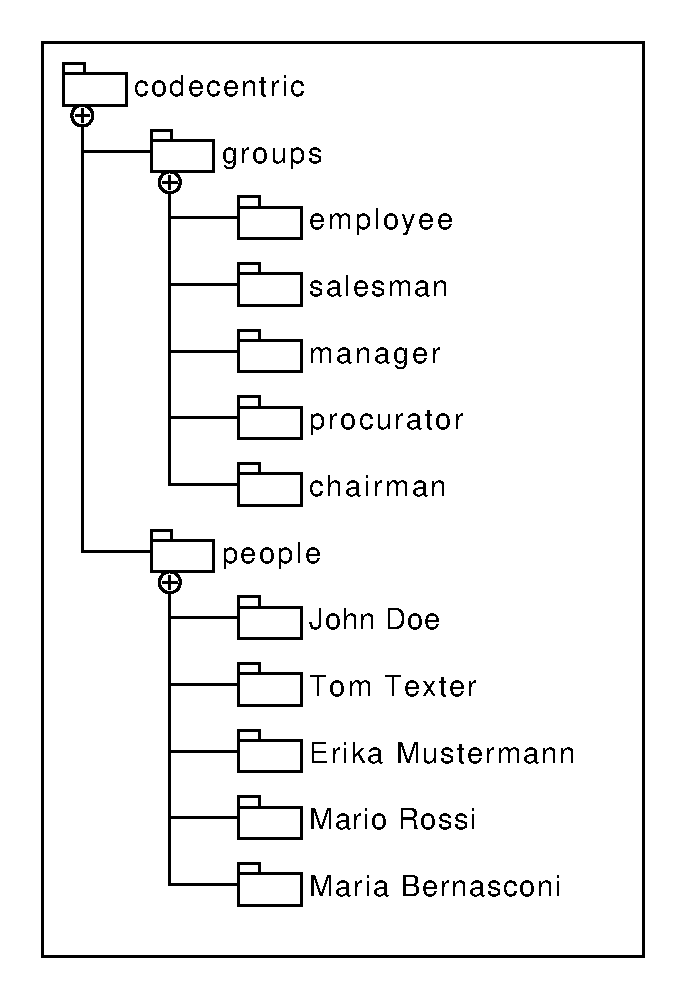
\includegraphics[height=8cm]{./implementation/images/ldap.pdf}
	\centering
	\caption{Structure of the Lightweight Directory Access Protocol Server}
	\label{fig:ldap}
\end{figure}

The connection to the server is done with \textit{Spring Boot}. Therefore three components are needed: A configuration class, entity classes that represent the different elements stored at the server, and repository interfaces that define the requests, which are made to the server regarding a specific entity. The complete class structure can be seen in figure \ref{fig:ldapMock}.

Due to the fact that an embedded server is used, it is not possible to test the logic with data from the \gls{ldap} server without starting the complete application. Therefore, the server connections, which are represented through repositories, are mocked with the framework \textit{Mockito}.

\section{Enterprise Resource System Connection}
Due to the fact that there is currently no \gls{erp} available, the decision was made to simulate it completely. Therefore, the implementation generates test data and stores them inside lists. Furthermore, only one file for signing is available, which is used to simulate all document types that should be processed inside the current project. Within the data it is ensured, that all possible scenarios could be simulated based on the new signing guideline presented in table \ref{tab:overviewTargets}. \newline
As test data for the company members, the same user names as in the user management are used to keep the data consistent for the complete system.

The testing of the logic has a simple structure, due to the fact that nothing needs to be mocked. But due to time constraints not all functionalities given through the interface are implemented, because until now they were not part of the \textit{User Stories} that should be implemented. The methods for getting the document itself and to store the signed document are not implemented and tested.


\section{Rule Set}
For the rule set implementation several options exist to store the signing rules. For the prototype, the decision was made to do it with a \gls{sql} \gls{db}, instead of using a file with \textit{JavaScript Object Notation} or an \gls{xml} file. The reason is that \textit{Spring Boot} offers the possibility to use an embedded \gls{sql} \gls{db}. Therefore, two files need to exist in the resource directory of the application: a \gls{sql} schema and a data \gls{sql} file. For an \gls{xml} data storage three files need to be created: a schema, a data type and a data file. Furthermore, a complete \gls{xml} reader needs to be developed to read the stored data. Therefore, the decision was made to use a \gls{sql} \gls{db}. \newline
With the usage of an embedded \gls{db} the setup work of the application is reduced, due to the fact that the \textit{Spring Boot} application always creates the \gls{db} when starting the application. This leads to the benefit that no extra \gls{db} server needs to be created and set up, even in the situation a demonstration is given on a different computer. \newline
As \gls{db} engine \textit{H2} is used, because it was advised by employees of \gls{cc} that often work with \textit{Spring Boot}. The benefit is the \textit{Java} based implementation of it, so that no extra software need to be installed beside of \textit{Java}.

The figure \ref{fig:db} presents the schema of the \gls{db} structure in an \textit{Entity Relation Diagram}. Differently from the design described in section \ref{sec:ruleRequest} there are six tables instead of five, but this is related to the constraints given through a relational \gls{db} and a \gls{sql} \gls{db} is mostly a relational \gls{db} \parencite{rdbsql2018}. The sixth table is the connection for the signing groups positions. In general the stored information should be simple structured to identify the different rules and related data.

\begin{figure}[h!]
	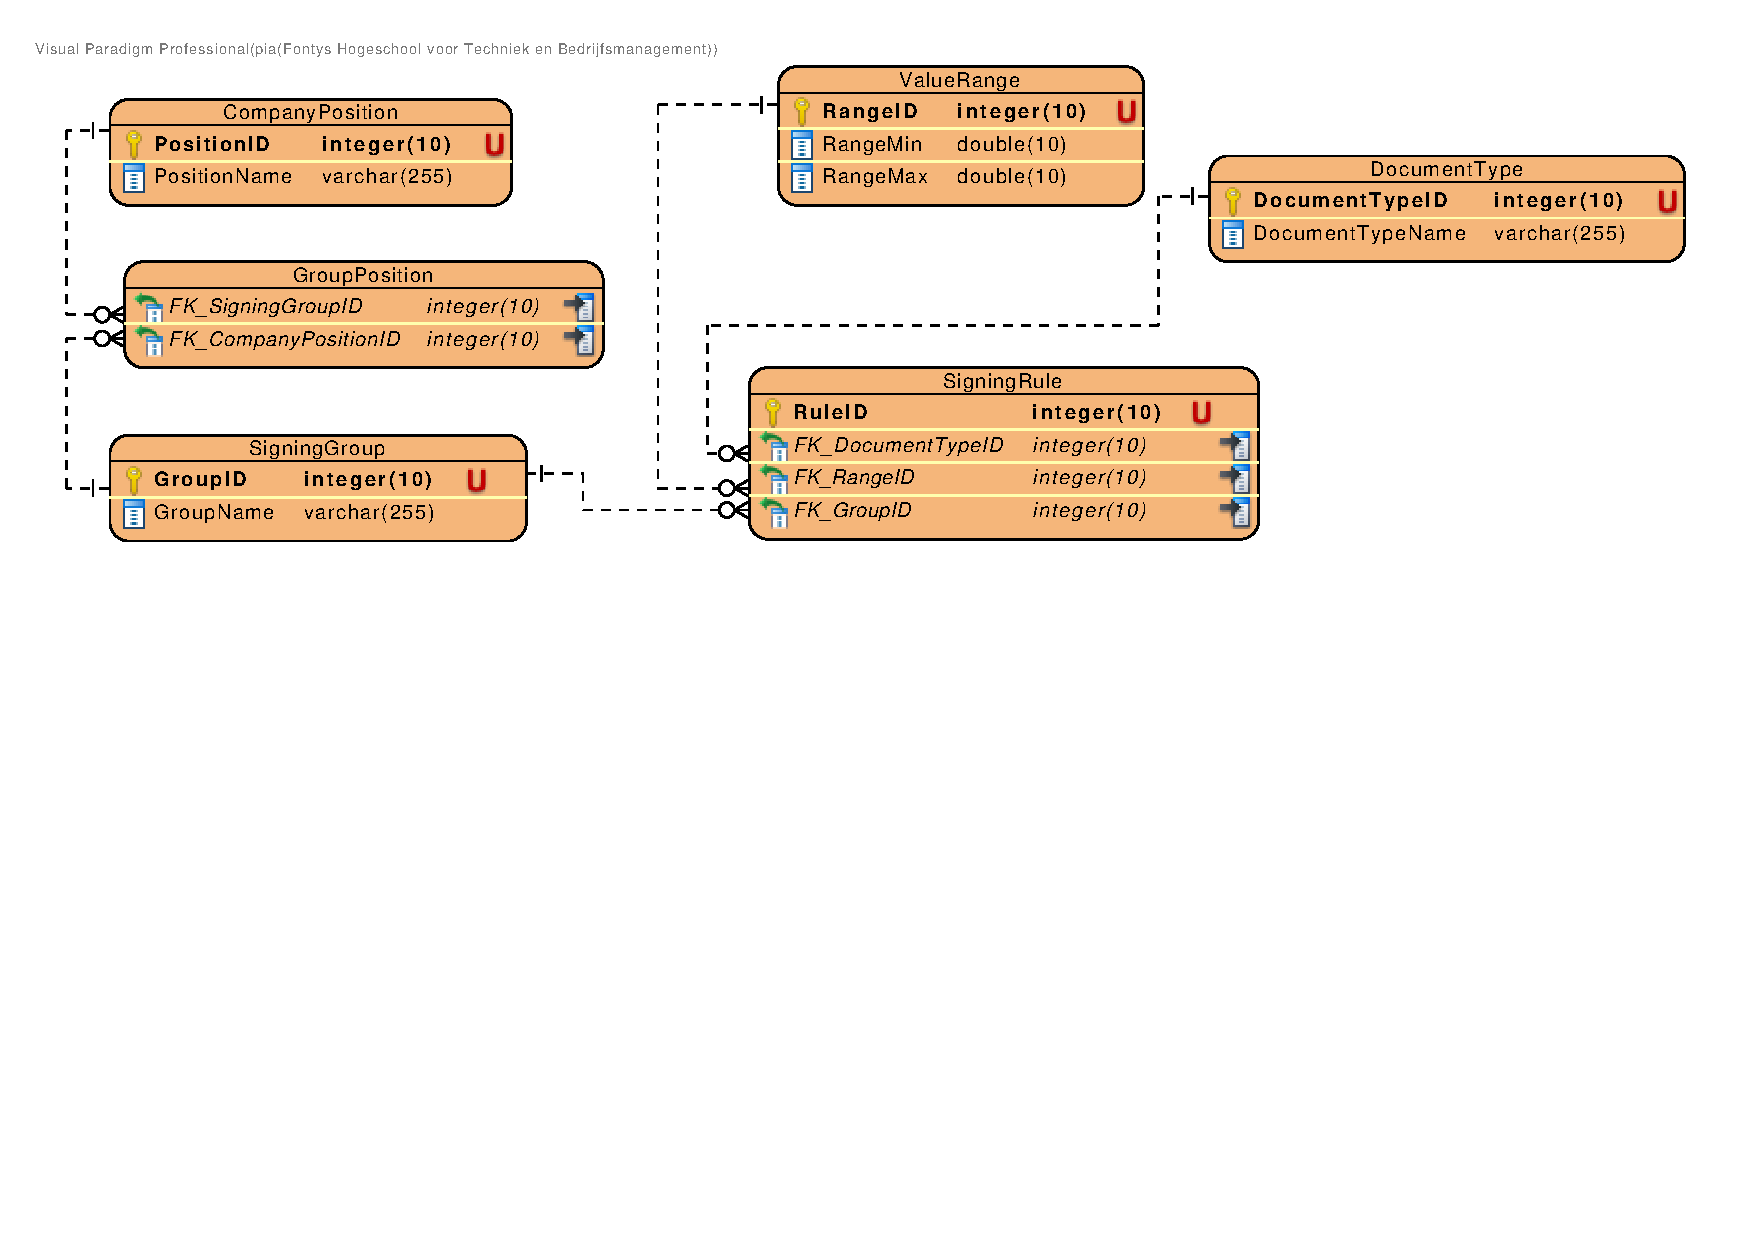
\includegraphics[width=\linewidth]{./implementation/images/db.pdf}
	\centering
	\caption{Entity Relation Diagram of the Rule Set Implementation}
	\label{fig:db}
\end{figure}

Besides the data storage, an implementation of the described algorithm from section \ref{sec:ruleRequest} is done. The complete class structure can be seen in figure \ref{fig:dbMock}. In general the code follows the structure given by the defined algorithm shown in appendix \ref{mathCode}, but at one point it has a customization. That is at the point in which the signing groups are sorted based on the size of the group. \newline
Inside this implementation no direct sorting is done, because that would take too much time and resources. Instead the option was developed to have an integer that represents the current minimum group size and a list that stores the groups with the smallest size. At the beginning of each new request it gets the highest integer value possible in the \textit{Java} environment. Then the following code is executed:

\begin{lstlisting}[language=Java,caption={Store signing group based on its size},captionpos=b]
if (compareList.size() < curent_min) {
curent_min = compareList.size();
returnList.clear();
returnList = iterateOverList(returnList, compareList);
} else if (compareList.size() == curent_min) {
returnList = iterateOverList(returnList, compareList);
}
\end{lstlisting}

The \textit{returnList} is the list that stores the signing groups and \textit{compareList} contains all positions of a signing group. The method \textit{iterateOverList()} only requests the name of the positions belonging to the group, because they are given previously with their identification number and for the later processing in the core system the name is required. \newline
In the case that the group size is smaller than the already stored value, all previously stored groups will be removed from the list and the smaller group is added. Otherwise if the size is equal to the current smallest groups, the group will be added to them.

Important to notice is, that it is expected, that there is no overlap within the different value ranges given to one document type, because the implementation does not care about this and takes the first value range that fits the requirements. \newline
Another important aspect to show up is that the tests also have to be mocked, because the used embedded \gls{db} is only created at the start of the complete application. This is one big disadvantage by using an embedded \gls{db}. For testing the framework \textit{Mockito} was used to mock the classes representing the connection to the \gls{db}. But due to a complex data logic the mocking of the data was extended and the effort the same as creating a complete new \gls{db} with a new stored data set.
 

\section{Signing System Connection}
For the prototype a connection to the \textit{DocuSign} tool should be created. A developer accounts exists which could be used for development and prototyping. Therefore, an account needs to be created for free so the \glspl{sdk} or the \gls{rest} \gls{api} can be used. But the constraint is, that it is only send to a demo environment and the received documents will be branded as such, and therefore are not approved by the law \parencite{docusign2018developer}. \newline
Due to time issues there will be no implementation, because the general setup with the previous requirements took more time than expected. But instead an advice will be given in chapter \ref{ch:advice}. 